\documentclass[tikz]{standalone}

\begin{document}
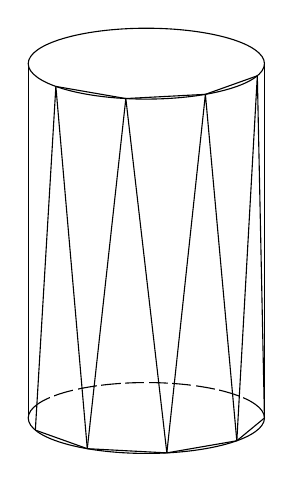
\begin{tikzpicture}[scale=1.5]
  \draw (0, 0) ellipse (1 and 0.3);
  \draw (-1, 0) -- (-1, 3);
  \draw (1, 0) -- (1, 3);
  \foreach \x in {-0.8, -0.6, ..., 0.8} {
    \draw[ultra thick, white] (\x, 0) -- (\x, 0.5);
  }
  \foreach \x in {0, -40, ..., -120} {
    \draw ({cos(\x)}, {0.3 * sin(\x)}) --
      ({cos(\x - 20)}, {3 + 0.3 * sin(\x - 20)}) --
      ({cos(\x - 40)}, {0.3 * sin(\x - 40)});
  }
  \draw[fill=white] (0, 3) ellipse (1 and 0.3);
  \foreach \x in {0, -40, ..., -120} {
    \draw ({cos(\x)}, {0.3 * sin(\x)}) --
      ({cos(\x - 40)}, {0.3 * sin(\x - 40)});
  }
  \foreach \x in {-40, -80, -120} {
    \draw ({cos(\x - 20)}, {3 + 0.3 * sin(\x - 20)}) --
      ({cos(\x + 20)}, {3 + 0.3 * sin(\x + 20)});
  }
\end{tikzpicture}
\end{document}
